\documentclass[aspectratio=169,11pt]{beamer}
\usetheme{default}
\usecolortheme{default}
\setbeamertemplate{navigation symbols}{}
\setbeamertemplate{footline}{\hfill\scriptsize\insertframenumber\,/\,\inserttotalframenumber\hspace{6pt}\vspace{4pt}}
\definecolor{accent}{HTML}{2A78D6}
\setbeamercolor{frametitle}{fg=accent}
\setbeamercolor{title}{fg=accent}
\setbeamercolor{structure}{fg=accent}
\setbeamerfont{frametitle}{series=\bfseries}
\usepackage{booktabs,graphicx,tikz}
\usetikzlibrary{arrows.meta,positioning}
\graphicspath{{../results/figures/}}
\tikzset{box/.style={draw, rounded corners=3pt, align=center, minimum height=0.95cm, text width=2.25cm, fill=#1!12, draw=#1!60!black},
  arr/.style={-{Stealth[length=2mm]}, thick, gray!70!black}}


\title{EdgeBot}
\subtitle{A voice-commanded warehouse mobile manipulator\\RL navigation $\cdot$ IK manipulation $\cdot$ Conversational AI $\cdot$ Edge deployment}
\author{Mehul Khanna}
\institute{UCS760 -- Edge AI and Robotics: Reinforcement Learning \& Conversational AI\\Thapar Institute of Engineering and Technology}
\date{November 2026}

\newcommand{\tbl}[1]{\resizebox{\linewidth}{!}{\input{generated/#1.tex}}}

\begin{document}
\frame{\titlepage}

\begin{frame}{Problem and idea}
\begin{columns}[T]
\column{0.55\linewidth}
\begin{itemize}
\item Warehouse robots must \textbf{navigate} among shelves, \textbf{manipulate} items precisely and take
\textbf{spoken instructions} from non-programmers.
\item EdgeBot implements the whole UCS760 syllabus as \textbf{one working system}, not separate exercises.
\item Every component is \textbf{measured on held-out data} and \textbf{exported for edge hardware}.
\end{itemize}
\vspace{6pt}
\textit{``Move the red box from shelf A to the conveyor''}\\
$\rightarrow$ ASR $\rightarrow$ intent + slots $\rightarrow$ plan $\rightarrow$ drive $\rightarrow$ pick $\rightarrow$ drive
$\rightarrow$ place $\rightarrow$ spoken reply.
\column{0.45\linewidth}
\small
\resizebox{\linewidth}{!}{\begin{tabular}{@{}ll@{}}
\toprule
Syllabus unit & EdgeBot module\\
\midrule
MDP, DP, MC, TD & warehouse grid MDP\\
Gym, DQN, PPO & JetBot navigation\\
RL for vision & pixel-based DQN\\
Manipulation, IK & 3-DOF arm workcell\\
Pick-n-place, assembly & lab tasks\\
NLP, BERT, slot filling & JointBERT + KD\\
ASR, TTS & Whisper, Piper\\
GPU, Jetson deployment & ONNX + INT8\\
\bottomrule
\end{tabular}}
\end{columns}
\end{frame}

\begin{frame}{Architecture}
\centering
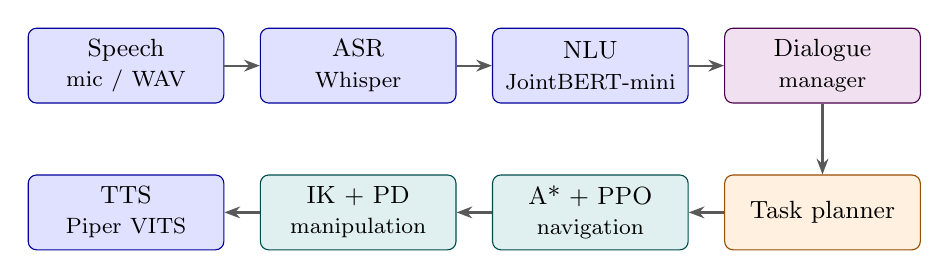
\begin{tikzpicture}[node distance=0.45cm and 0.45cm, every node/.style={font=\small}]
\node[box=blue] (mic) {Speech\\ \footnotesize mic / WAV};
\node[box=blue, right=of mic] (asr) {ASR\\ \footnotesize Whisper};
\node[box=blue, right=of asr] (nlu) {NLU\\ \footnotesize JointBERT-mini};
\node[box=violet, right=of nlu] (dm) {Dialogue\\ \footnotesize manager};
\node[box=orange, below=0.9cm of dm] (plan) {Task planner};
\node[box=teal, left=of plan] (nav) {A* + PPO\\ \footnotesize navigation};
\node[box=teal, left=of nav] (man) {IK + PD\\ \footnotesize manipulation};
\node[box=blue, left=of man] (tts) {TTS\\ \footnotesize Piper VITS};
\draw[arr] (mic)--(asr); \draw[arr] (asr)--(nlu); \draw[arr] (nlu)--(dm); \draw[arr] (dm)--(plan);
\draw[arr] (plan)--(nav); \draw[arr] (nav)--(man); \draw[arr] (man)--(tts);
\end{tikzpicture}
\vspace{10pt}
\begin{itemize}\small
\item Hierarchical navigation: \textbf{A*} global plan on an inflated grid, \textbf{learned PPO policy} as the reactive local controller.
\item Learn what is hard to model (unknown obstacles); compute what is known exactly (arm kinematics).
\item Policy, NLU and TTS run in \textbf{ONNX Runtime}; ASR in \textbf{CTranslate2} (FP16 GPU / INT8 CPU).
\end{itemize}
\end{frame}

\begin{frame}{RL foundations: warehouse grid MDP}
\begin{columns}[T]
\column{0.5\linewidth}
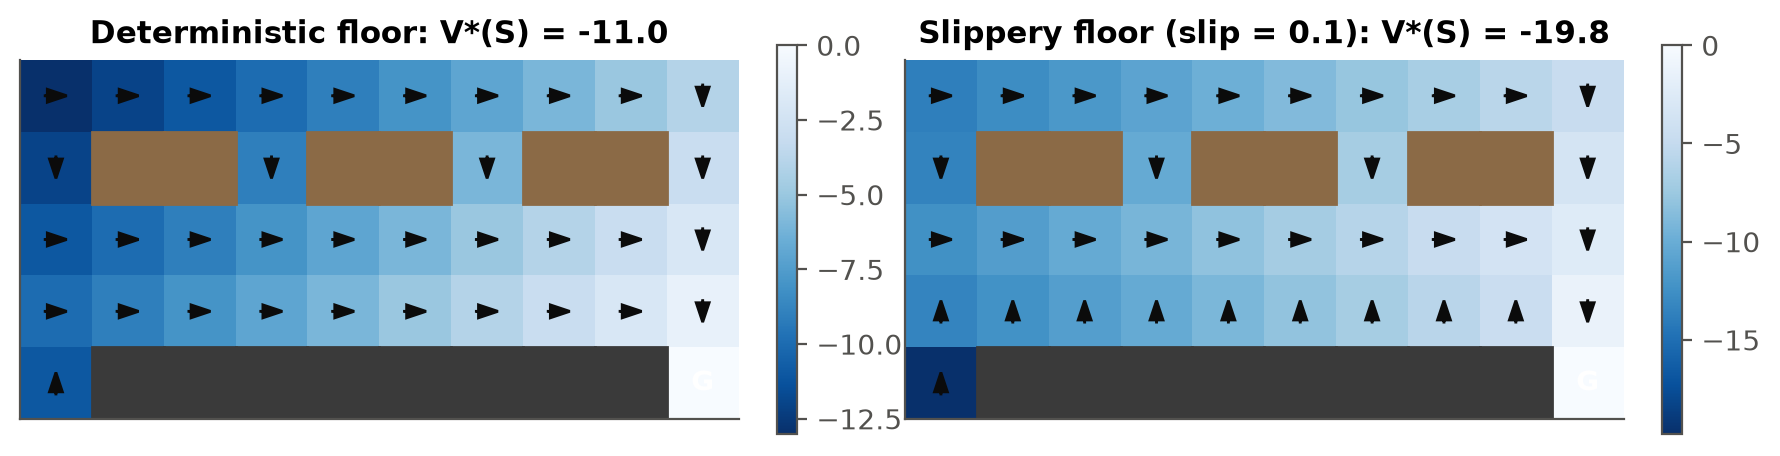
\includegraphics[width=\linewidth]{dp_value_policy.png}\\[2pt]
\tbl{tab_dp}
\column{0.5\linewidth}
\small
\begin{itemize}
\item Oil spill on the shortest route: $-100$ and reset (Cliff Walking).
\item VI and PI agree to $10^{-8}$; slippery floor $\Rightarrow$ optimal policy keeps one row away.
\item \textbf{SARSA} learns the safe route, \textbf{Q-learning} the optimal edge route (with poorer online return): on- vs.\ off-policy.
\end{itemize}
\tbl{tab_control}
\end{columns}
\end{frame}

\begin{frame}{Learning curves and TD prediction}
\begin{columns}[c]
\column{0.6\linewidth}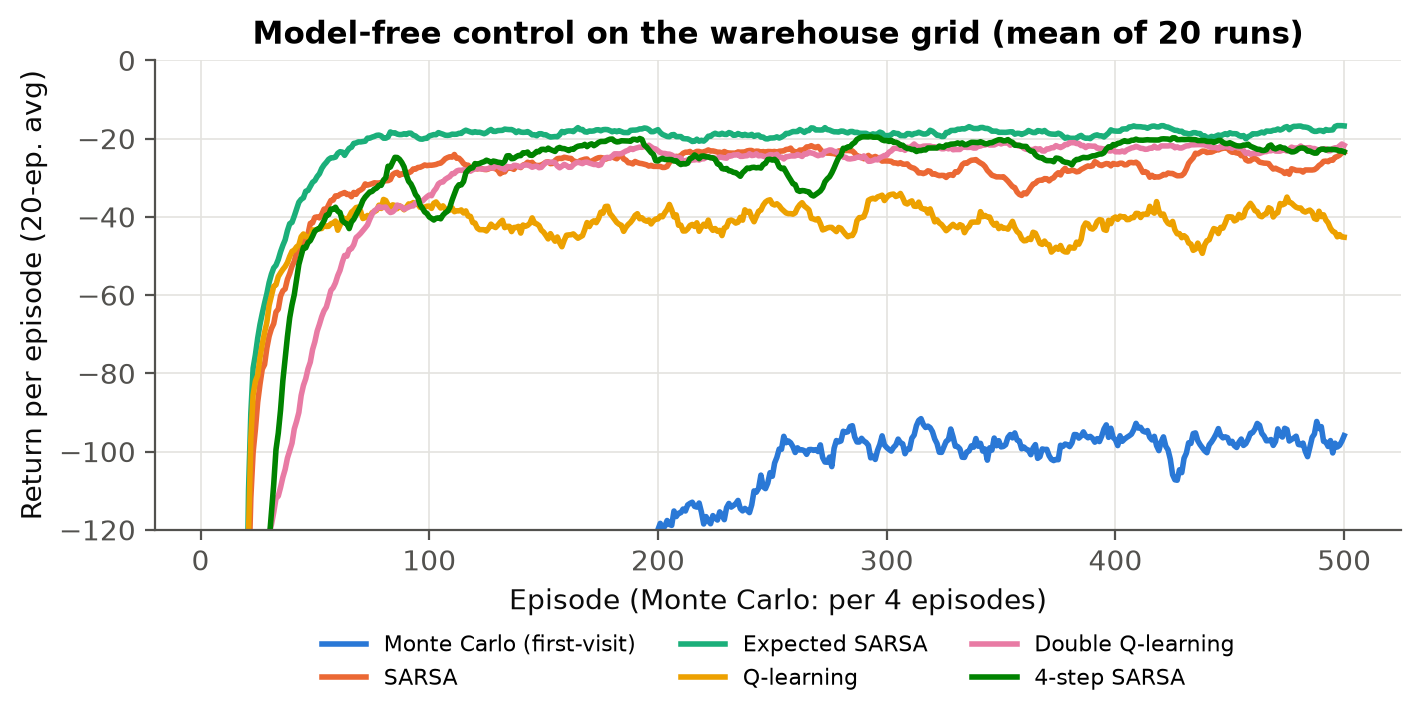
\includegraphics[width=\linewidth]{tabular_learning_curves.png}
\column{0.4\linewidth}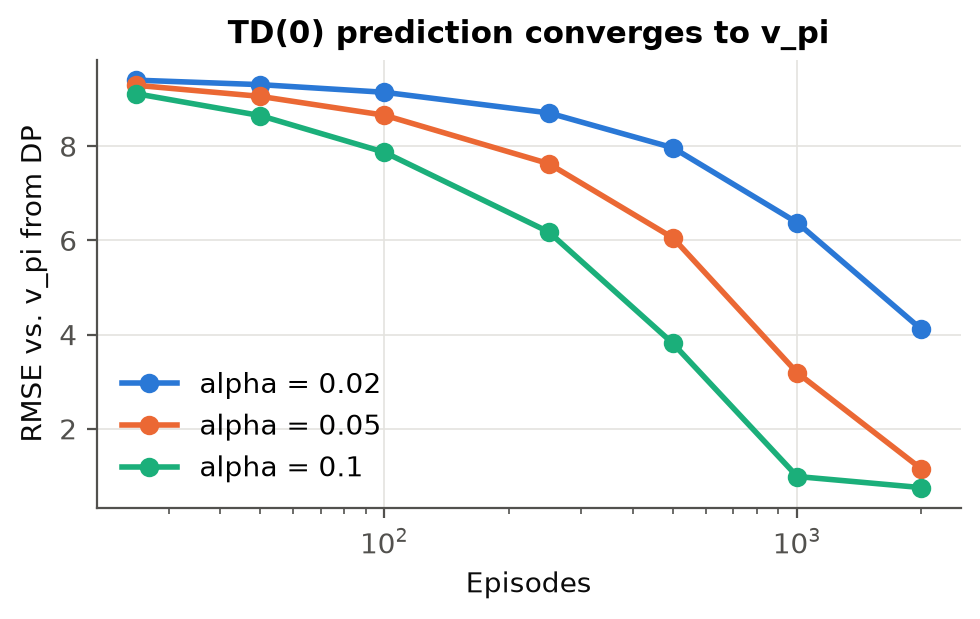
\includegraphics[width=\linewidth]{td0_prediction.png}
\end{columns}
\vspace{6pt}
\centering\small 20 independent seeds per method. TD(0) converges to $v_\pi$ computed by Dynamic Programming.
\end{frame}

\begin{frame}{JetBot navigation in continuous space}
\begin{columns}[T]
\column{0.52\linewidth}
\small
\begin{itemize}
\item Gymnasium environment, unicycle kinematics at 10\,Hz, \textbf{new random warehouse every episode}.
\item Observations: 24-beam lidar + goal (29-D), or $2{\times}64{\times}64$ egocentric images.
\item \textbf{PPO}: Gaussian policy, GAE, clipped surrogate, KL early stop, truncation bootstrap.
\item \textbf{DQN}: replay, target net, Double + Dueling, CNN torso for pixels.
\end{itemize}
\column{0.48\linewidth}
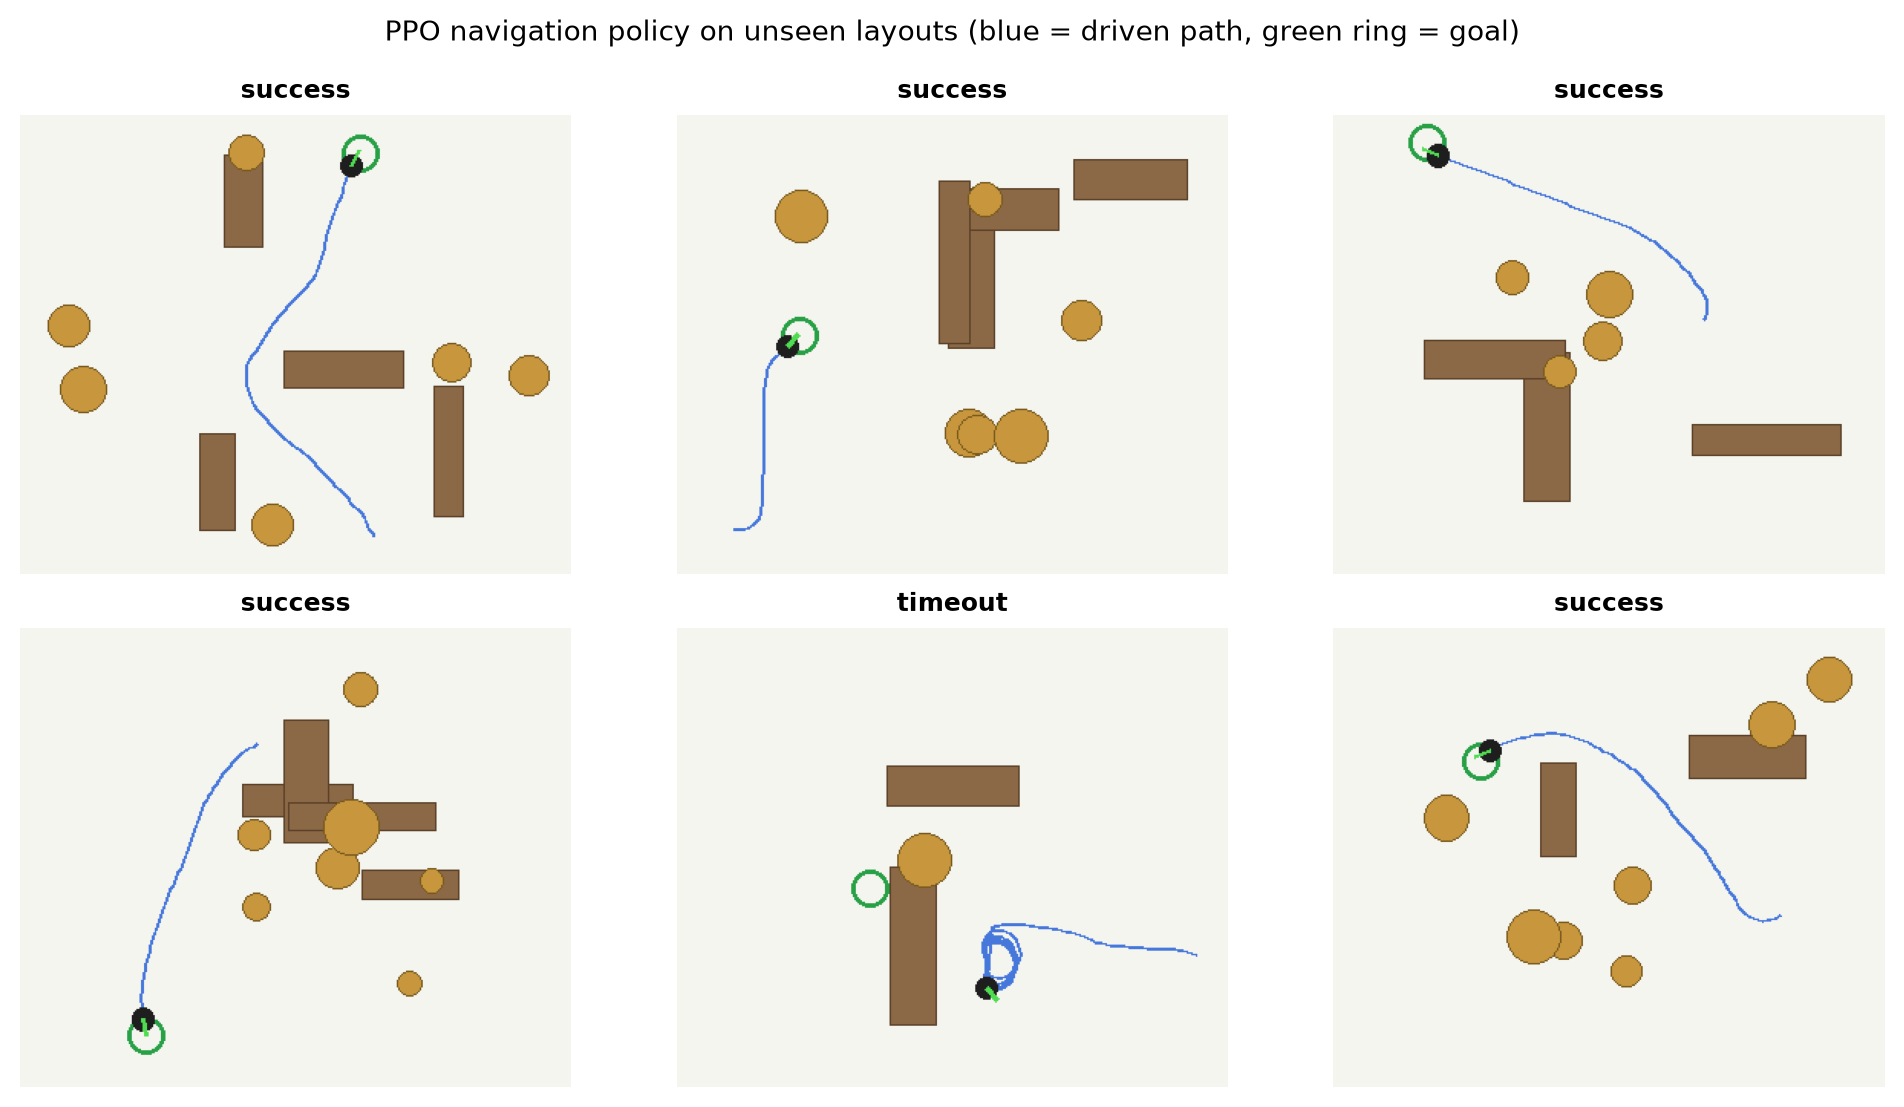
\includegraphics[width=\linewidth]{nav_trajectories.png}
\end{columns}
\vspace{4pt}
\tbl{tab_nav}
\end{frame}

\begin{frame}{Navigation training}
\centering
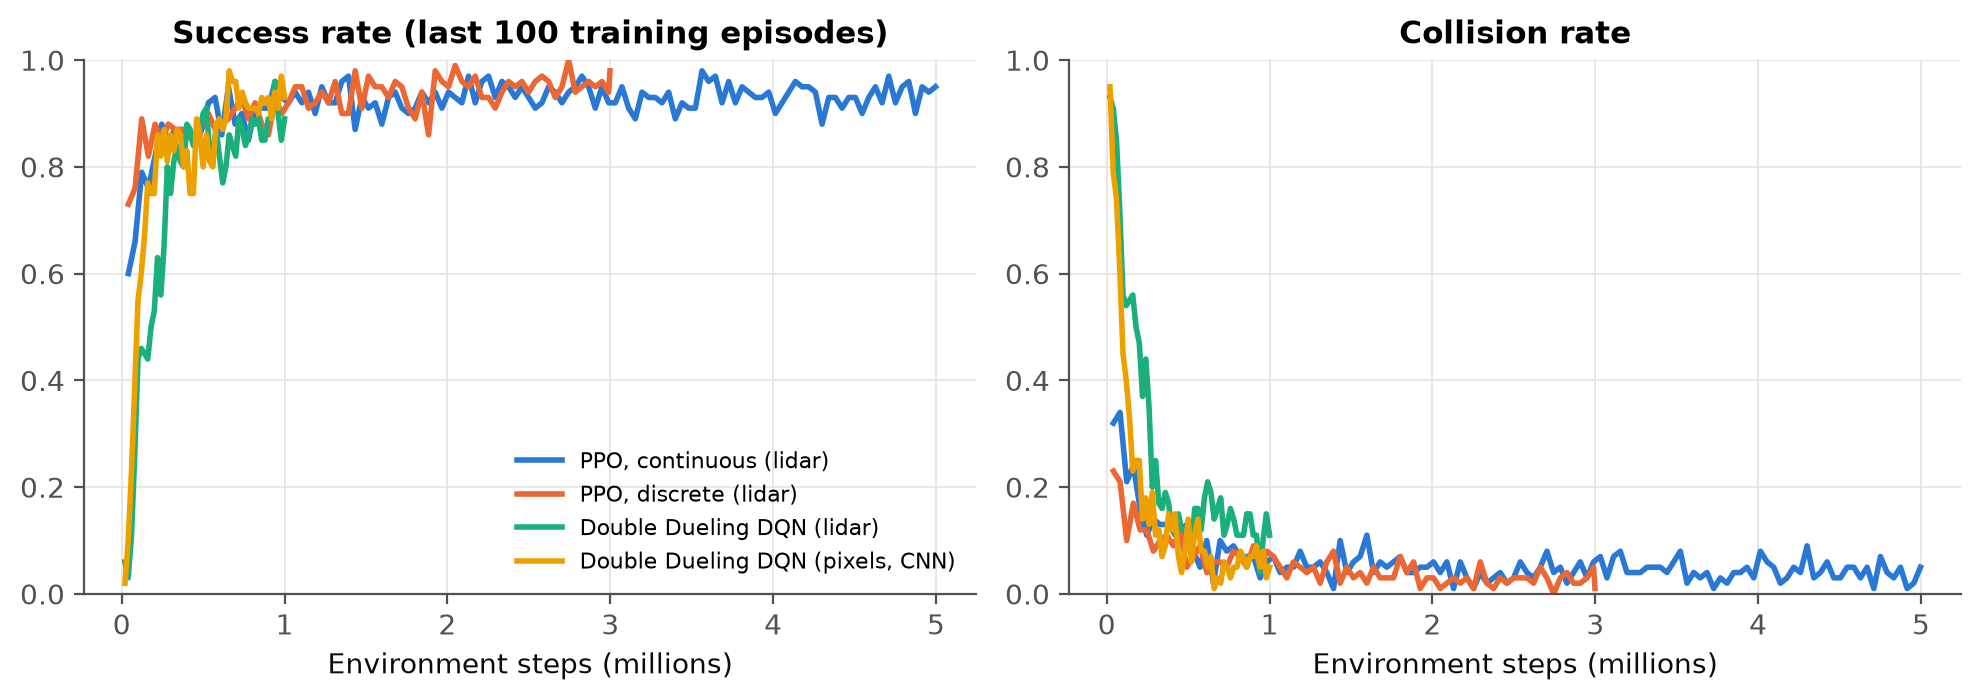
\includegraphics[width=0.9\linewidth]{nav_learning_curves.png}\\[4pt]
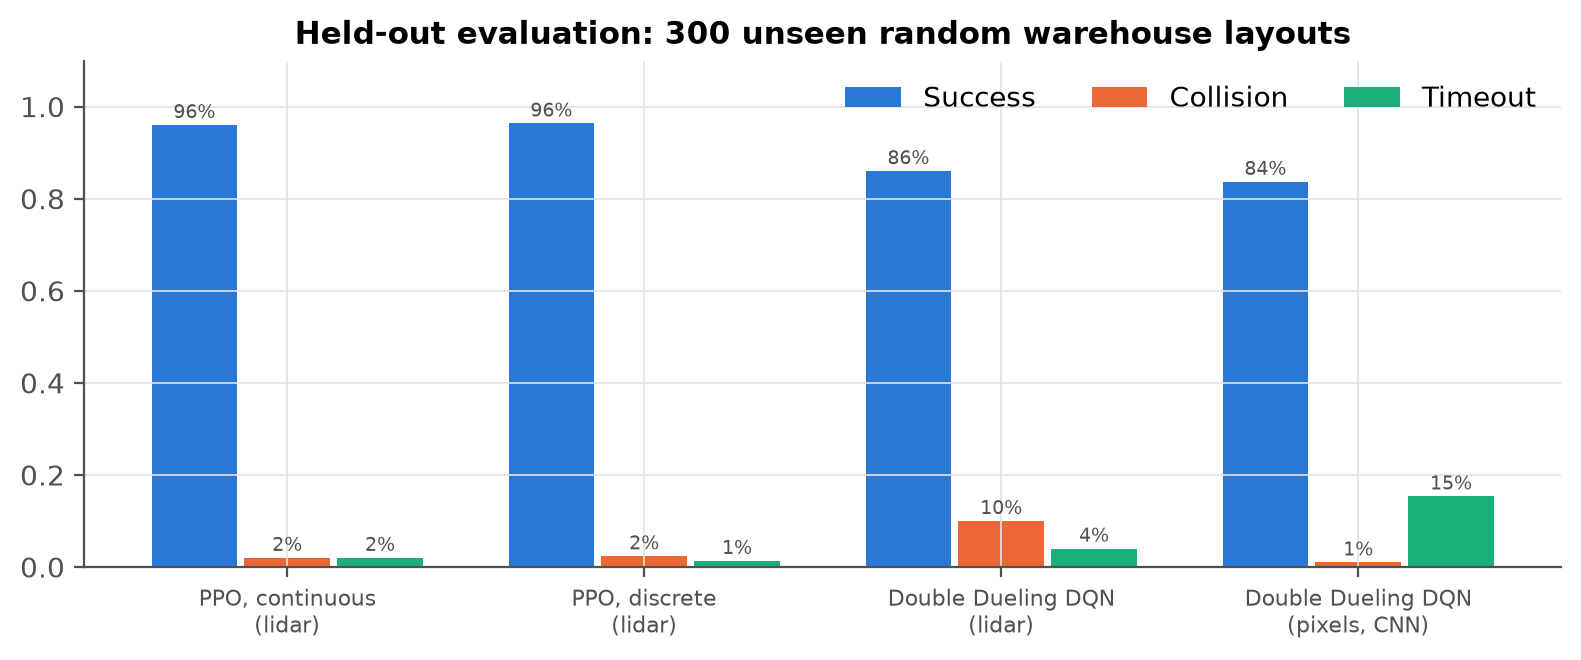
\includegraphics[height=0.36\textheight]{nav_eval_bars.png}
\end{frame}

\begin{frame}{Manipulation: kinematics, IK and control}
\begin{columns}[T]
\column{0.5\linewidth}
\small
\begin{itemize}
\item Planar RRR arm, \textbf{DH} forward kinematics, analytic Jacobian (checked by finite differences).
\item \textbf{Closed-form IK} (law of cosines, elbow-up) vs.\ \textbf{damped least squares}.
\item Minimum-jerk quintic joint trajectories, Cartesian straight-line approach.
\item PD + feed-forward + gravity compensation on a torque-limited joint model.
\end{itemize}
\tbl{tab_ik}
\column{0.5\linewidth}
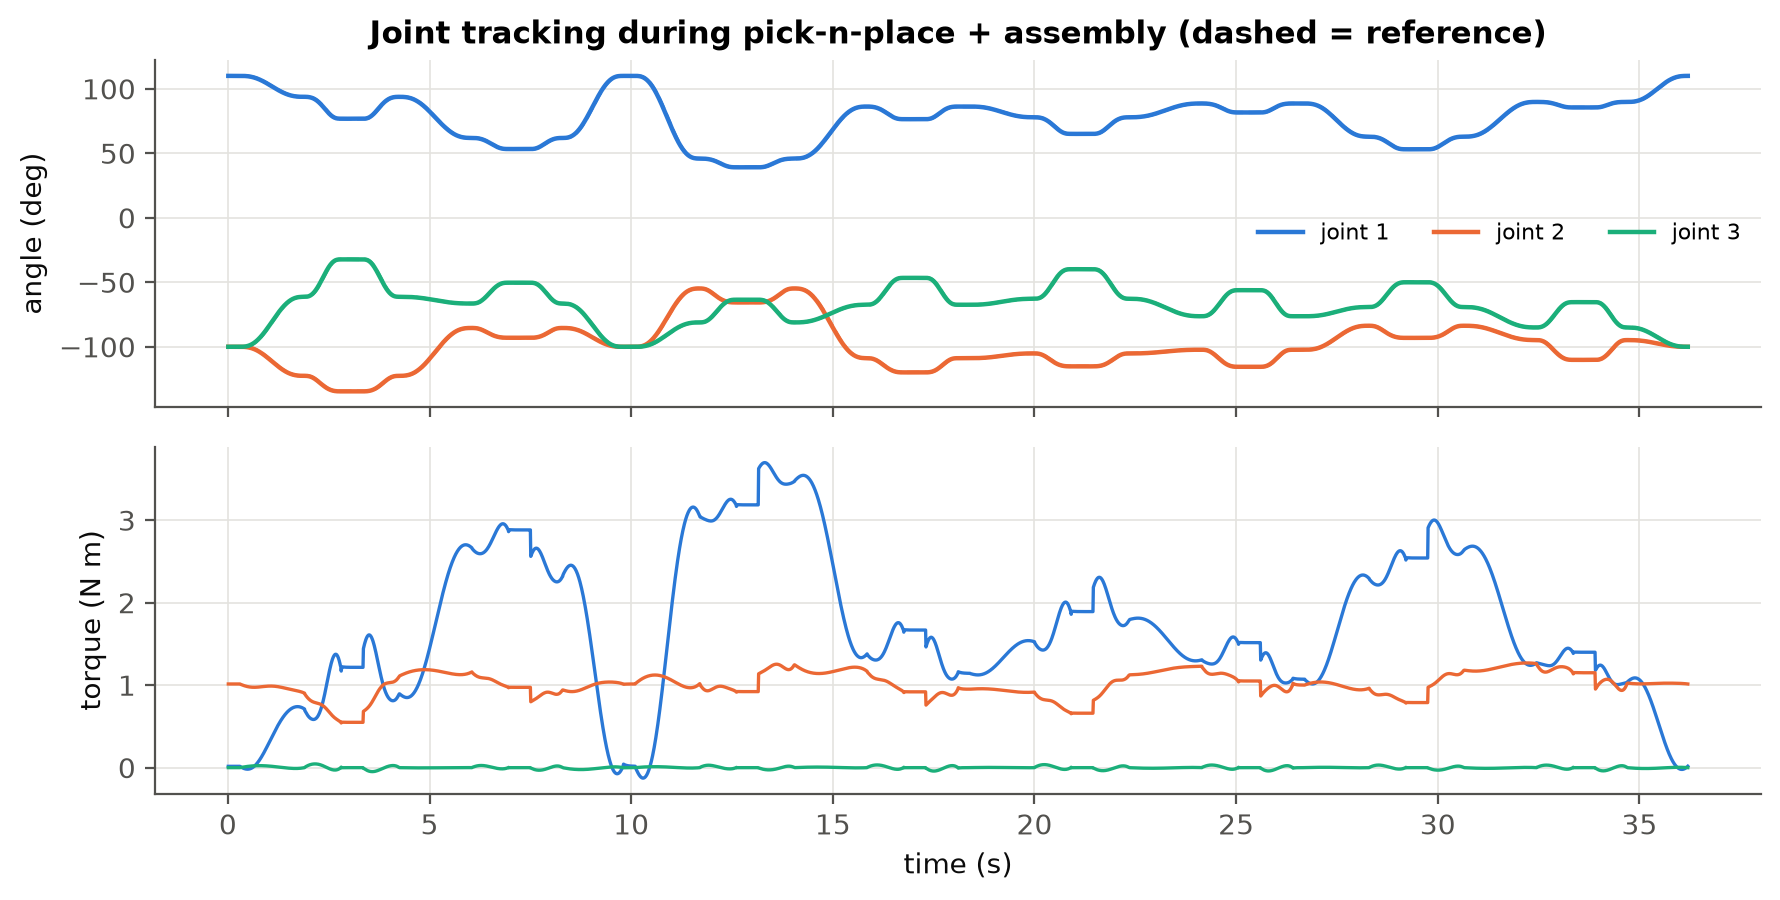
\includegraphics[width=\linewidth]{joint_tracking.png}
\end{columns}
\end{frame}

\begin{frame}{Labs: pick-n-place and object assembly}
\begin{columns}[T]
\column{0.5\linewidth}
\small
\begin{itemize}
\item Grasp only if the gripper is within 12\,mm; released blocks fall onto their support, so success is \textbf{simulated, not assumed}.
\item 100 randomised trials per task.
\item \textbf{Task learning}: PPO learns reaching from reward, compared against analytic IK.
\end{itemize}
\tbl{tab_manip}
\column{0.5\linewidth}
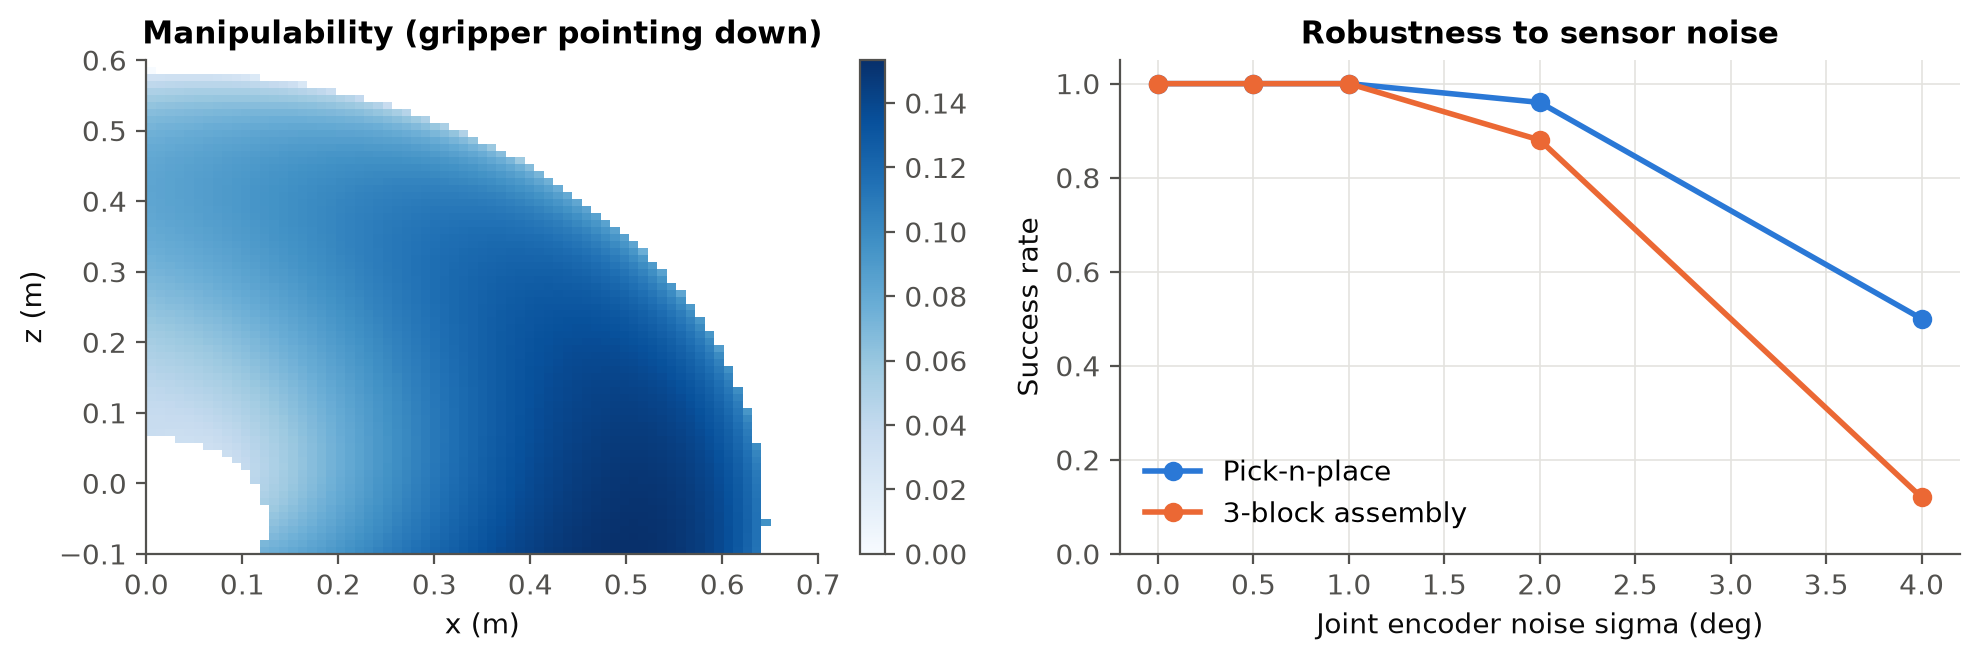
\includegraphics[width=\linewidth]{manipulation_analysis.png}
\end{columns}
\end{frame}

\begin{frame}{Conversational AI: NLU}
\begin{columns}[T]
\column{0.46\linewidth}
\small
\begin{itemize}
\item 9 intents + BIO slots.
\item Test set: \textbf{sentence templates never seen in training}, clean and with ASR noise.
\item \textbf{JointBERT-mini}: 2-layer Transformer, [CLS] intent head, word + char-CNN embeddings.
\item \textbf{Teacher}: DistilBERT fine-tuned jointly.
\item \textbf{Distillation}: MLM augmentation (TinyBERT) + soft-label KL, $T=2$.
\end{itemize}
\column{0.54\linewidth}
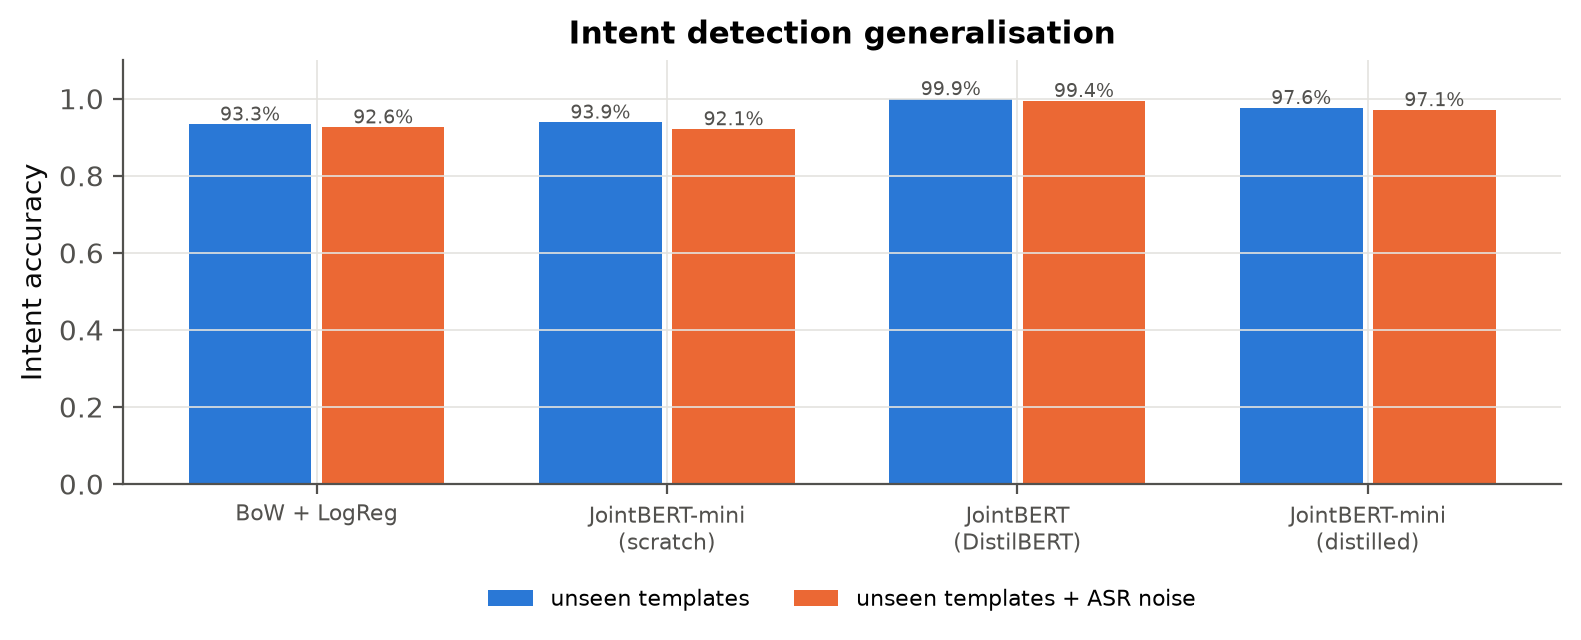
\includegraphics[height=0.36\textheight]{nlu_comparison.png}
\end{columns}
\vspace{2pt}
{\centering\resizebox{0.8\linewidth}{!}{\begin{tabular}{lrrrrr}
\toprule
Model & Params & Intent acc. & Slot F1 & Frame acc. & Intent (noisy) \\
\midrule
BoW + logistic regression & -- & 93.3\% & -- & -- & 92.6\% \\
JointBERT-mini (scratch) & 0.32M & 93.9\% & 99.0\% & 91.4\% & 92.1\% \\
JointBERT (DistilBERT fine-tuned) & 66.38M & 99.9\% & 100.0\% & 99.9\% & 99.4\% \\
JointBERT-mini (distilled, deployed) & 0.49M & 97.6\% & 99.3\% & 97.6\% & 97.1\% \\
\bottomrule
\end{tabular}
}\par}
\end{frame}

\begin{frame}{Conversational AI: speech in the loop}
\begin{columns}[T]
\column{0.5\linewidth}
\small
\begin{itemize}
\item \textbf{ASR}: Whisper-base (encoder--decoder), domain prompt; compared conceptually with the CTC family Jasper / QuartzNet / CitriNet.
\item \textbf{TTS}: Piper VITS (single network, ONNX) vs.\ the two-stage Tacotron2 + WaveGlow.
\item 150 held-out commands spoken by TTS, + white noise, $\rightarrow$ ASR $\rightarrow$ NLU.
\end{itemize}
\tbl{tab_speech_rtf}
\column{0.5\linewidth}
\tbl{tab_voice}\\[8pt]
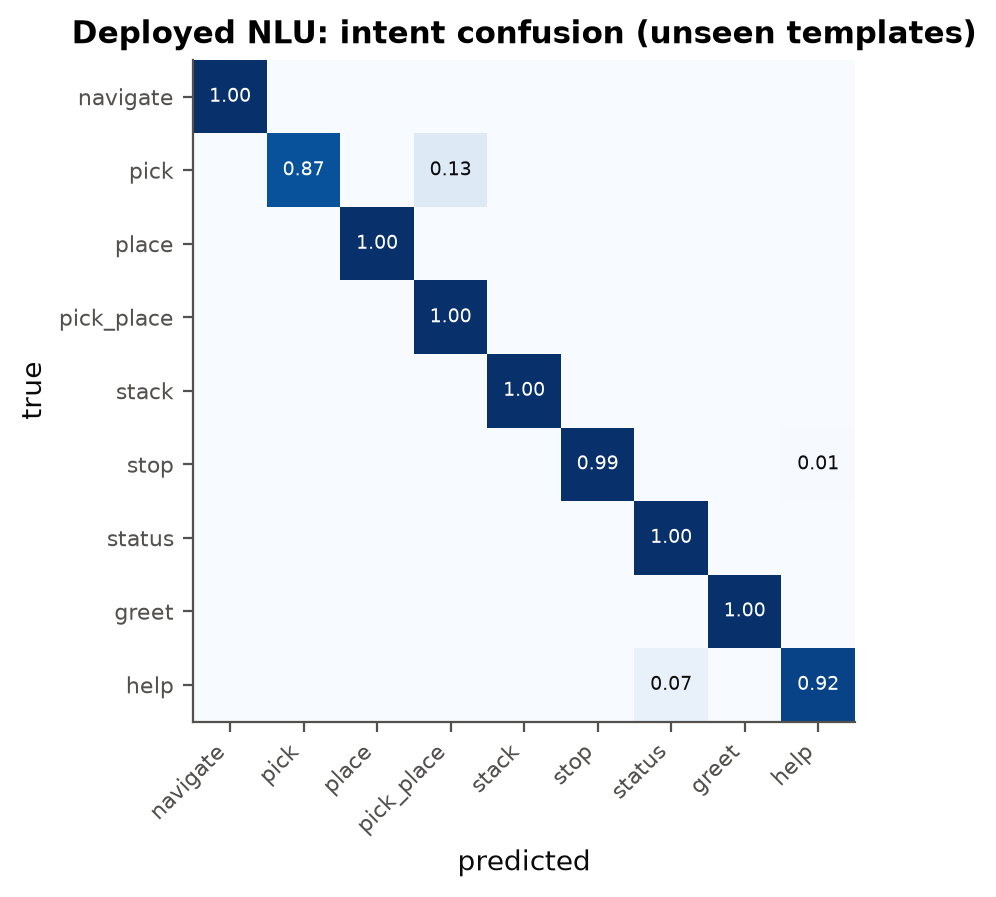
\includegraphics[width=0.85\linewidth]{nlu_confusion.png}
\end{columns}
\end{frame}

\begin{frame}{Edge deployment}
\begin{columns}[T]
\column{0.4\linewidth}
\small
\begin{itemize}
\item Export to \textbf{ONNX} (TensorRT's input on Jetson), verified against PyTorch.
\item Batch-1, \textbf{single CPU thread} latency: the controller's operating point.
\item Small nets: GPU launch overhead $>$ compute $\Rightarrow$ CPU + ONNX Runtime wins.
\item INT8: 3--4$\times$ smaller; PPO and NLU keep accuracy.
\item CNN policy: per-tensor INT8 hurts; \textbf{calibrated static per-channel} recovers it.
\end{itemize}
\column{0.6\linewidth}
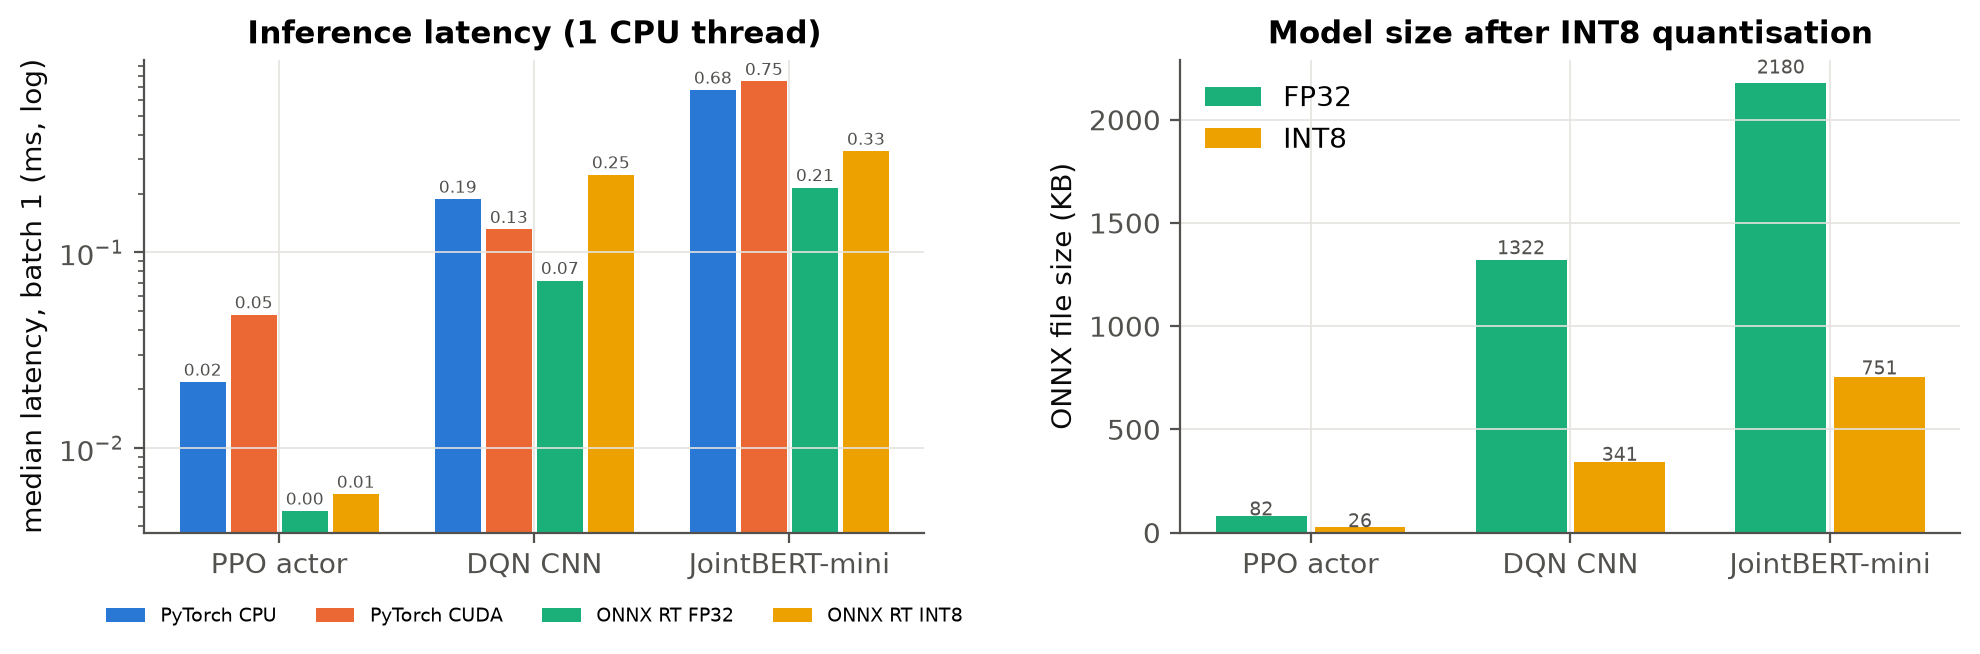
\includegraphics[width=\linewidth]{edge_benchmark.png}\\[4pt]
\resizebox{\linewidth}{!}{\begin{tabular}{lrr}
\toprule
Task metric & ONNX FP32 & ONNX INT8 \\
\midrule
PPO navigation success & 95.0\% & 95.0\% \\
DQN (pixels) navigation success & 81.0\% & 42.0\% \\
NLU frame accuracy & 97.6\% & 97.5\% \\
\bottomrule
\end{tabular}
}\\[4pt]
\resizebox{\linewidth}{!}{\begin{tabular}{lrrr}
\toprule
DQN (pixels) variant & Size (KB) & ORT latency (ms) & Nav. success \\
\midrule
FP32 & 1322 & 0.072 & 81.0\% \\
INT8 dynamic, per-tensor & 341 & 0.249 & 42.0\% \\
INT8 dynamic, per-channel & -- & -- & 65.0\% \\
INT8 static QDQ, per-channel, calibrated & 347 & 0.044 & 74.0\% \\
\bottomrule
\end{tabular}
}
\end{columns}
\end{frame}

\begin{frame}{Integrated demo}
\begin{columns}[T]
\column{0.38\linewidth}
\small
\begin{enumerate}
\item ``hello jetbot''
\item ``move the red box from shelf A to the conveyor''
\item ``pick up the box'' $\rightarrow$ \emph{Which colour?}
\item ``the blue one''
\item ``put it on the packing station''
\item ``stack the red, green and blue blocks at the workbench''
\item ``what is your status''
\item ``go back to the charging dock''
\end{enumerate}
\texttt{python scripts/run\_demo.py --voice}
\column{0.62\linewidth}
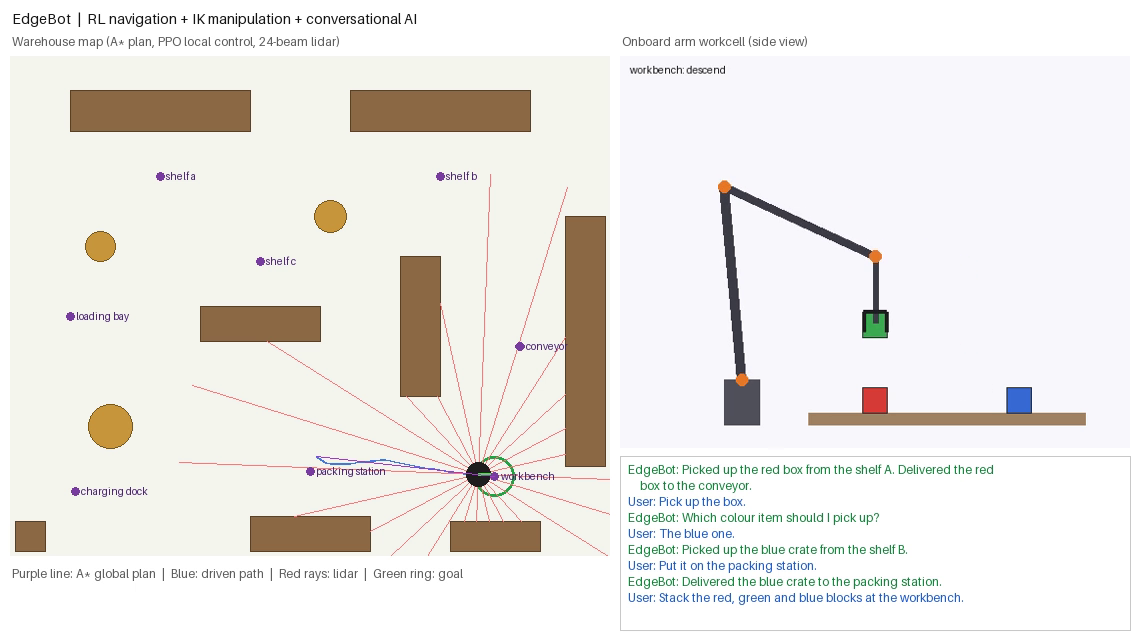
\includegraphics[width=\linewidth]{demo_frame.png}
\end{columns}
\end{frame}

\begin{frame}{Conclusions}
\begin{itemize}
\item One coherent edge-AI robot covering \textbf{every syllabus unit and lab}, with held-out evaluation throughout.
\item RL is used where models are unknown (navigation), classical robotics where they are exact (IK);
the reaching study quantifies that choice.
\item Pretraining + distillation is what makes a 0.5\,M-parameter NLU generalise to unseen phrasing.
\item All controllers run in about a millisecond or less per call on one CPU thread; speech runs faster than real time.
\item \textbf{Next}: TensorRT on Jetson Orin, sensor noise and domain randomisation for sim-to-real, 6-DOF arm, real user speech.
\end{itemize}
\vspace{8pt}
\centering\small Code, results and this deck: \texttt{github.com/MrMehulkhanna/edgebot}
\end{frame}
\end{document}
